\title{Midterm 2 for Computer Logic and Circuit Design: PHYS306/COSC330}
\author{Dr. Jordan Hanson - Whittier College Dept. of Physics and Astronomy}
\date{\today}
\documentclass[10pt]{article}
\usepackage[a4paper, total={18cm, 27cm}]{geometry}
\usepackage{outlines}
\usepackage[sfdefault]{FiraSans}
\usepackage{hyperref}
\usepackage{graphicx}
\begin{document}
\maketitle

\textit{This take-home midterm exam is open-note.  It is due Monday, May 14th, 2018 in SLC 212 mail slot by end of the day.}

\section{Karnaugh maps and POS/SOP expressions}
\begin{enumerate}
\item A remote weather station meant to alert residents of tornados appears to be malfunctioning.  Four sensors pass data to a machine learning algorithm trained to send a FALSE signal when there is a tornado and remain TRUE otherwise.  There is a temperature sensor, a windspeed sensor, a humidity sensor, and a barometer.  There must be some electrical problem, because the system sends a FALSE with no tornado present under the following conditions.  1) The temperature sensor is powered, and the other sensors are off.  2) The temperature and barometer are powered, but the other sensors are off.  3) All sensors are off.  4) The barometer is powered, and the other sensors are off.  Determine the simplest condition that leads to this erroneous FALSE signal when powering the sensors.  \\ \vspace{4cm}
\item Suppose you remove the two sensors that are malfunctioning by causing the machine learning algorithm to report FALSE, indicating a tornado when there is none.  Now, the machine learning system sends TRUE (correct, since there's no tornado around), when both sensors are powered.  A replacement wind sensor is added.  Later that month, a tornado approaches the area around the station.  The wind, temperature and barometer sensors are activated remotely.  The following conditions produce a FALSE machine learning output.  1) The temperature, wind and barometer sensors are powered, and 2) the temperature and wind sensors are powered while the barometer is not powered.  Determine the simplest logic expression representing this state.  Which device is malfunctioning? \\ \vspace{3cm}
\end{enumerate}

\section{Combinational logic with gates, tables, and expressions}
\begin{enumerate}
\begin{figure}
\centering
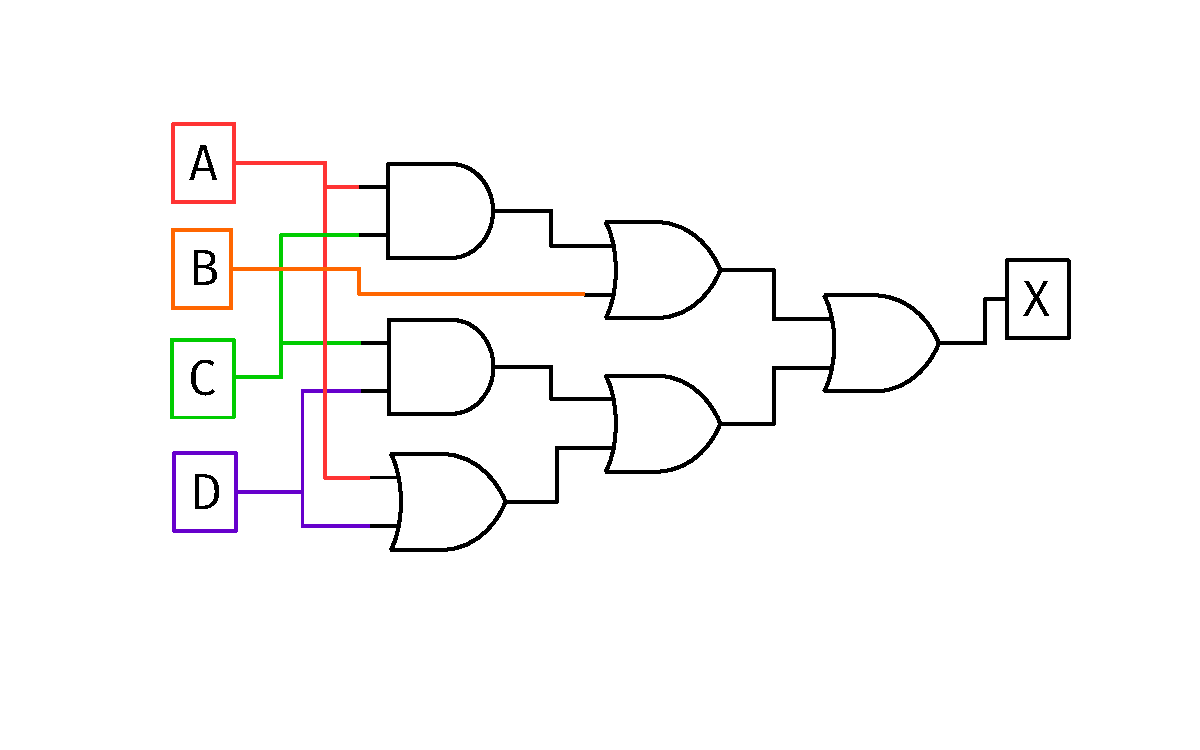
\includegraphics[width=0.5\textwidth,trim=2cm 3cm 2cm 2cm,clip=true]{figures/MultiGate3.pdf}
\caption{\label{fig:m3} A combinatorial logic circuit.}
\end{figure}
\item Implement the logic circuit in Fig. \ref{fig:m3} using only NAND gates. Draw a diagram and show that that the truth tables match. \\ \vspace{4cm}
\end{enumerate}

\end{document}
